\chapter{Dunnville sandstone characterization}\label{ch3:title}


This chapter presents a summary of geology, mineralogical composition and strength properties of Dunnville Sandstone. The results of simple tests such as uniaxial compression test and drained conventional triaxial tests on dry specimens are discussed and analyzed.

\section{Geology, mineralogy and properties of the Dunnville sandstone}

In this study, Dunnville sandstone was selected for the laboratory experiments due to its availability, known strength properties and its isotropic behavior at relatively high confining stresses. Indeed, previous experiments on Dunnville Sandstone showed an isotropic behavior under different conditions of triaxial testing \cite{Tarokh2016}. The following paragraphs provide a short summary of geological and mineralogical properties of Dunnville sandstone.

\subsection{Geological history}

Dunnville sandstone comes from Dunnville, in western Wisconsin. The rock quarry is located in a valley at the intersection of the Chippewa river and one of its affluent. Dunnville sandstone constituent materials were deposited during the Cambrian period when Wisconsin was submerged several times by a sea, enabling the deposition of a large amount of sediments. The consolidation and compaction of the deposited materials by glaciers during the Pleistocene Epoch geological time and the subsequent removal of ice due to melting and rise in ambient temperatures led to the development of highly over-consolidated sedimentary rocks in the region (i.e., Dunnville sandstone). Dunnville sandstone is a member of the Elk Mount Formation and particularly the Eau Claire group \cite{Ostrom1966}.

\subsection{Mineralogy}

Dunnville Sandstone is composed of 90\% of medium-grained quartz and a small amount of cementitious material and may be referred to as a quartz arenite. Other minerals are readily noticeable such as orange beds of alkali feldspars and biotite grains (Fig. \ref{fig3:1}). The elongated biotite crystals are disparately distributed in the rock matrix and oriented parallel to the bedding. The mineralogical composition of Dunnville sandstone performed by American Engineering Testing is summarized in Table \ref{tb3:mineralogy} \cite{Tarokh2016}. Dunnville sandstone is a highly porous and permeable rock, with a porosity of 29-30\% \cite{Tarokh2016}.

\begin{figure}[tb]
    \centering
    \includegraphics[width=0.4\columnwidth]{ch3/20191016_151842}
    \includegraphics[width=0.2\columnwidth]{ch3/20191017_105210}
    \caption{Dunnville sandstone mineralogy}
    \label{fig3:1}
\end{figure} 

\begin{table}[h]
    \centering
    \begin{tabular}{lc} \hline
        Mineral & Volume [\%] \\ \hline \hline
        Quartz & 90-95 \\ 
        Alkali Feldspar & 2-5 \\ 
        Biotite & 2-5 \\ 
        Plagioclase & Trace -1 \\ 
        Muscovite & Trace \\ 
        Clinozoisite & Trace \\ 
        Zircon & Trace \\ 
        Hematite & Trace \\ 
        Iron-oxide & 1-2 \\ \hline
    \end{tabular}
    \caption{Mineralogy of Dunnville Sandstone \cite{Tarokh2016}}
    \label{tb3:mineralogy}
\end{table}





The dry density and the P-Wave velocity through the rock were measured for all specimens tested in this study. The dry density $\rho$ is approximately $1910 \pm 30 \; \text{kg/m}^3$ and the P-wave velocity VP is $1825\pm 124 \; \text{m/s}$ . The wave travel time for evaluation of the P-wave velocity was measured perpendicular to the bedding planes in the tested specimens for uniaxial compression and drained conventional triaxial tests.

\section{Uniaxial compression test}

One uniaxial compression test was performed on Dunnville Sandstone, in order to determine Young’s modulus $E_i$ and the unconfined compressive strength $C_o$. These parameters are essential to understand the behavior of the rock and are used for the analysis of behavior in subsequent chapters.

\subsection{Specimen preparation}

A cylindrical specimen was already available from previous experiments. It was ground to ensure the ends were perpendicular to the specimen axis and dried prior to test in accordance with the ISRM suggested methods \cite{ISRM2015} and ASTM standard \cite{ASTM2019} [4]. A detailed description of the specimen preparation procedure will be presented in section \ref{ch3:specimen-prep}. This specimen respected the standard dimensions for a uniaxial test (i.e. $h\approx 2d$) with the following characteristics: $h = 95.70$ mm, $d = 50.76$ mm. Following Labuz and Bridell (1993) [5], stearic acid was applied to the specimen ends to reduce end friction and thereby to minimize the end effects.

\subsection{Procedure}

The test was performed using a \SI{1}{\mega\newton} MTS closed loop servo-hydraulic load frame (MTS System Corporation). The uniaxial compression test was stroke controlled to avoid sudden failure of the rock where a displacement rate of \SI{0.001}{\milli\meter\per\second} was used. The displacement of the load frame and the force applied to the specimen was recorded during the test.

A small seating load of ~1-2 kN was applied before the test initiated to ensure adequate contact between the loading platens and the specimen. The axial load was then increased until the achievement of ~ 50\% of the expected uniaxial compressive strength $C_o$ of the rock following by unloading to ~1-2 \si{kN}. The axial load was then increased until failure of the rock specimen was achieved. The test was continued until the load decreased to ~ 75\% of $C_o$. This loading-unloading cycle is used to determine the Young’s modulus $E_i$ of the rock after specimen displacements were corrected for the machine displacement.

For this test, the following stress path is considered: 

\begin{align}
    \sigma_1 = \sigma_a &\text{ with } \sigma_a > 0 \\
    \sigma_2 = \sigma_3 = \sigma_r   &\text{ with } \sigma_r = 0
\end{align}

\subsection{Results}

From the recorded axial displacement and force, the axial stress and the axial strain could be computed: 

\begin{align}
    \sigma_a &= \frac{F_a}{A} \\
    \epsilon_a &= \frac{u}{h}
\end{align}

Where:

\begin{description}
    \item[$\sigma_a$] : axial stress  [\si{\mega\pascal}]
    \item[$\epsilon_a$] : axial strain [-]
    \item[$A=\frac{d\pi^2}{4}$] : cross section area of the cylindrical specimen [\si{\milli\meter\squared}]
    \item[$F_a$] :  axial load applied through the load frame [\si{\newton}]
    \item[$u$] : axial displacement corrected for machine displacement [\si{\milli\meter}]
    \item[$h$]  length of the specimen [\si{\milli\meter}]
\end{description}

Fig \ref{fig3:2} present the stress-strain plot obtained from the uniaxial compression test. The uniaxial compressive strength of the rock specimen is calculated as: 


\begin{figure}[tb]
    \centering
    \includegraphics[width=\columnwidth]{ch3/ucs.pdf}
    \caption{Stress and Strain relationship for the uniaxial compression test}
    \label{fig3:2}
\end{figure} 

\begin{equation}
    C_o = \frac{F_\text{peak}}{A} = \sigma_{a,\text{peak}} = \SI{29.83}{\mega\pascal}
\end{equation}

The Young’s Modulus of the rock is computed using the loading-unloading cycle:

\begin{equation}
    E=\frac{\Delta\sigma}{\Delta\epsilon} = \SI{5860}{\mega\pascal}
\end{equation}

Fig \ref{fig3:3} presents the specimen after the test. The failed specimen showed a failure surface with a conical shape at \SI{63}{\degree}. 

\begin{figure}[tb]
    \centering
    \includegraphics[width=0.4\columnwidth]{ch3/ucs.png}
    \caption{Stress and Strain relationship for the uniaxial compression test}
    \label{fig3:3}
\end{figure} 

\section{Conventional Triaxial tests}\label{Conventional_Triaxial_tests}

Dunnville sandstone shear strength was determined using conventional triaxial tests (CT). Two types of CT tests were performed, namely, the conventional triaxial compression (CTC) and the conventional triaxial extension (CTE). For these tests, two of the principal stresses of the stress state are equal. The state of stress of the rock specimen is then simplified to a combination of the axial stress $\sigma_a$ and the radial stress $\sigma_r$. 

\subsection{Hoek-Franklin cell}

A Hoek -Franklin pressure cell was used to perform the conventional triaxial tests \cite{Franklin1970}. The maximum capacity of the cell is \SI{69}{MPa} and allows for the independent application of axial and radial stresses. The device is composed of a pressure vessel, a synthetic rubber membrane and two loading platens (Fig \ref{fig3:4}).

\begin{figure}[tb]
    \centering
    \includegraphics[width=0.4\columnwidth]{ch3/20191008_171805}
    \caption{Hoek-Franklin cell}
    \label{fig3:4}
\end{figure} 

The radial stress was applied using a fluid pressure system where confinement is provided using hydraulic oil. The fluid pressure system is composed of a microcontroller and a screw-type hydraulic intensifier that allows for confining pressure to be held constant throughout the test. The axial load is applied through steel platens with a \SI{1}{\mega\newton} MTS servo-hydraulic load frame (MTS System Corporation). The monitoring of the load frame and axial force measurement are done using a closed-looped and data acquisition system (Fig \ref{fig3:5}).

\begin{figure}[tb]
    \centering
    \includegraphics[width=0.4\columnwidth]{ch3/20190927_172117}
    \caption{Conventional triaxial test set up}
    \label{fig3:5}
\end{figure} 

A rubber membrane was used to isolate the specimen and the loading platens from the confining fluid, and to allow for radial and axial stresses to be applied independently. The membranes used herein have an inner diameter of \SI{32.0}{mm} and are \SI{85.0}{mm} in height (Fig \ref{fig3:6}).

\begin{figure}[tb]
    \centering
    \includegraphics[width=0.4\columnwidth]{ch3/ctc10}
    \caption{Membrane hosting the rock specimen in the Hoek-Franklin cell}
    \label{fig3:6}
\end{figure} 

\subsection{Specimen preparation} \label{ch3:specimen-prep}

Rock cores were obtained from a block of Dunnville sandstone. The specimens were prepared following ASTM Standard Practice D4543-19 \cite{ASTM2019}. In preparation of the test specimens, particular attention was given to (i) the straightness of the elements on the cylindrical surface, (ii) flatness of the end bearing surfaces and (iii) perpendicularity of the end surfaces with the respect to axis of the core. The following describes the procedure used in preparation of the specimens:

\begin{enumerate}
    \item \emph{Cutting and grinding of the end surfaces}: for the purpose of sealing, the specimen dimensions should match that of the Hoek-Franklin cell membrane. The core diameters ranged from \SIrange{30.2}{30.6}{mm}. The specimens were cut and ground to reach a height h of approximately  \SI{85.0}{mm} The specimens were cut using a saw table and ground using a diamond impregnated wheel. Finally, a precision table was used to ensure that specimen ends were perpendicular to the specimen axis. The final height h of the specimens ranged from \SIrange{75.7}{81.8}{mm} 
    \item \emph{Drying}: all the specimens were oven dried at \SI{150}{\celsius} for at least 24 hours before the tests to ensure drained conditions existed during the triaxial tests
    \item \emph{Minimizing end friction}: the ends and cylindrical surface of the specimens were coated with stearic acid \cite{ASTM2019}. This lubricant was used to reduce frictional effects between the membrane and the specimen.
\end{enumerate}

In addition to standard geometrical preparation, one specimen (i.e. TC 9 at $\sigma_r = \SI{5}{MPa}$) was equipped with a strain gages rosette where axial and transverse strains were measured (Fig \ref{fig3:7}). The procedure for the strain gages sets up had to be executed with much care to avoid damaging it. All the tools used in the process were cleaned with acid and neutralizer before touching the strain gage. Due to the high porosity of the Dunnville Sandstone, the surface of the rock had to be coated with the same epoxy that was used to attach the component. The surface of the specimen was then cleaned using xylene and the strain gage was attached using M-Bond 200 adhesive.

\begin{figure}[tb]
    \centering
    \includegraphics[width=0.4\columnwidth]{ch3/straingage.png}
    \caption{Strain Gage set up on a CTC specimen}
    \label{fig3:7}
\end{figure} 

\subsection{Conventional Triaxial Compression test} \label{ch3:Conventional-Triaxial-Compression-test}

The following procedure was followed to setup and run the conventional triaxial compression tests:

\begin{enumerate}
    \item The specimen was inserted in the Hoek-Franklin cell. The cell was held in a horizontal position and hydraulic oil was inserted to ensure no entrapped air existed in the annulus between the cell walls and the membrane.
    \item The pressure cell-specimen-loading platen assembly was then placed inside the load frame and seating stress of  $\sigma_a \approx \SI{1}{MPa}$ was applied to the specimen to ensure adequate contact between the specimen and the platens. To ensure small deviatoric stresses, we also applied a $\sigma_r \approx \SI{1}{MPa}$. It is noted that this condition corresponds to a hydrostatic stress state (i.e. $\sigma_a = \sigma_r = \SI{1}{MPa}$ ).
    \item The axial ($\sigma_a$) and radial ($\sigma_r$) stresses were then increased hydrostatically until the desired confining pressure ($\sigma_r$) was achieved. In so doing, a stress increment of \SI{\sim 5}{MPa} was consistently used.
    \item Once the desired confining pressure (i.e., radial pressure $\sigma_r$) was reached, the deviatoric loading was initiated by maintaining the radial stresses ($\sigma_r$) while axial stresses ($\sigma_a$) were increased until failure was achieved. It is noted that all tests were stroke controlled where a displacement rate of \SI{0.001}{\meter\per\second} was used. The stress path applied during the test can be summarized as follow:
\end{enumerate}

\begin{align}
    \sigma_1 = \sigma_a &\text{ with } \sigma_a > 0 \\
    \sigma_2 = \sigma_3 = \sigma_r   &\text{ with } \sigma_r = 0 \\
    \sigma_a > \sigma_r &
\end{align}

$\sigma_1$, $\sigma_2$  and $\sigma_3$ are the principal stresses of the stress state; respectively major, intermediate and minor stress. The radial stress was kept constant at the desired confining pressure using the hydraulic intensifier, while the axial stress increased through the stroke of the load frame. 

\subsection{Conventional Triaxial Compression test}

The following procedure was followed to setup and run the conventional triaxial extension tests:

\begin{enumerate}
    \item The same device and tests preparation, as the those previously explained for the conventional triaxial compression tests, were used for the conventional triaxial extension tests (i.e., see steps 1-3 in Section \ref{ch3:Conventional-Triaxial-Compression-test}).
    \item In a conventional triaxial extension test, however, the axial load is decreased as opposed to increasing the axial stress in triaxial compression tests. 
    \item This test was stroke controlled and a displacement rate of \SI{0.001}{\meter\per\second} was used consistently. The radial stress was kept constant at the desired confining pressure using the hydraulic intensifier, while the axial stresses decreased through the displacement of the load frame. The stress path applied during the test can be summarized as follow:
\end{enumerate}

\begin{align}
    \sigma_1 = \sigma_2 = \sigma_r   &\text{ with } \sigma_r = 0 \\
    \sigma_3 = \sigma_a &\text{ with } \sigma_a < 0 \\
    \sigma_a < \sigma_r &
\end{align}

$\sigma_1$, $\sigma_2$  and $\sigma_3$ re the principal stresses of the stress state; respectively major, intermediate and minor stress. The radial stress was kept constant at the desired confining pressure using the hydraulic intensifier, while the axial stress increased through the stroke of the load frame. 

\subsection{Tests results}


Five conventional triaxial compression tests (i.e. $\sigma_r = $ \SIlist{5;10;20;40;60}{MPa}) and three conventional triaxial extension tests (i.e., $\sigma_r = $ \SIlist{35;40;60}{MPa} ) were performed. The test results are summarized in Table \ref{tb3:CTC-CTE-results} and the stress-strain relationships for all tests are shown in Fig \ref{fig3:8}

\begin{table}
    \centering
    \begin{tabular}{cccccccc}
        \hline 
        Test & $\sigma_1$ [\si{MPA}] & $\sigma_2$ [\si{MPA}] &$\sigma_3$ [\si{MPA}] & $p$ [\si{MPA}] & $q$ [\si{MPA}] & $\theta$ [\si{\degree}] & $E_i$ [\si{MPA}] \\
        \hline
        \hline
        TC 9  & 49.43 & 5  & 5    & 19.81 & 44.43 & 0  & 5861  \\ 
        TC 0  & 61.43 & 10 & 10   & 27.95 & 51.43 & 0  & 6407  \\ 
        TC 5  & 91.08 & 20 & 20   & 44.72 & 71.08 & 0  & 7014  \\ 
        TC 8  & 127.3 & 40 & 40   & 65.73 & 87.30 & 0  & 6687  \\ 
        TC 10 & 151.1 & 60 & 60   & 88.12 & 91.10 & 0  & 6842  \\ 
        \hline
        \hline
        TE 3  & 35    & 35 & 3.96 & 24.64 & 31.08 & 60 & 7922  \\ 
        TE 1  & 40    & 40 & 4.50 & 27.89 & 36.34 & 60 & 8390  \\ 
        TE 2  & 60    & 60 & 9.68 & 43.01 & 50.98 & 60 & 8695  \\
        \hline
    \end{tabular}
    \caption{Summary of CTC and CTE tests results}
    \label{tb3:CTC-CTE-results}
\end{table}

\begin{figure}[tb]
    \centering
    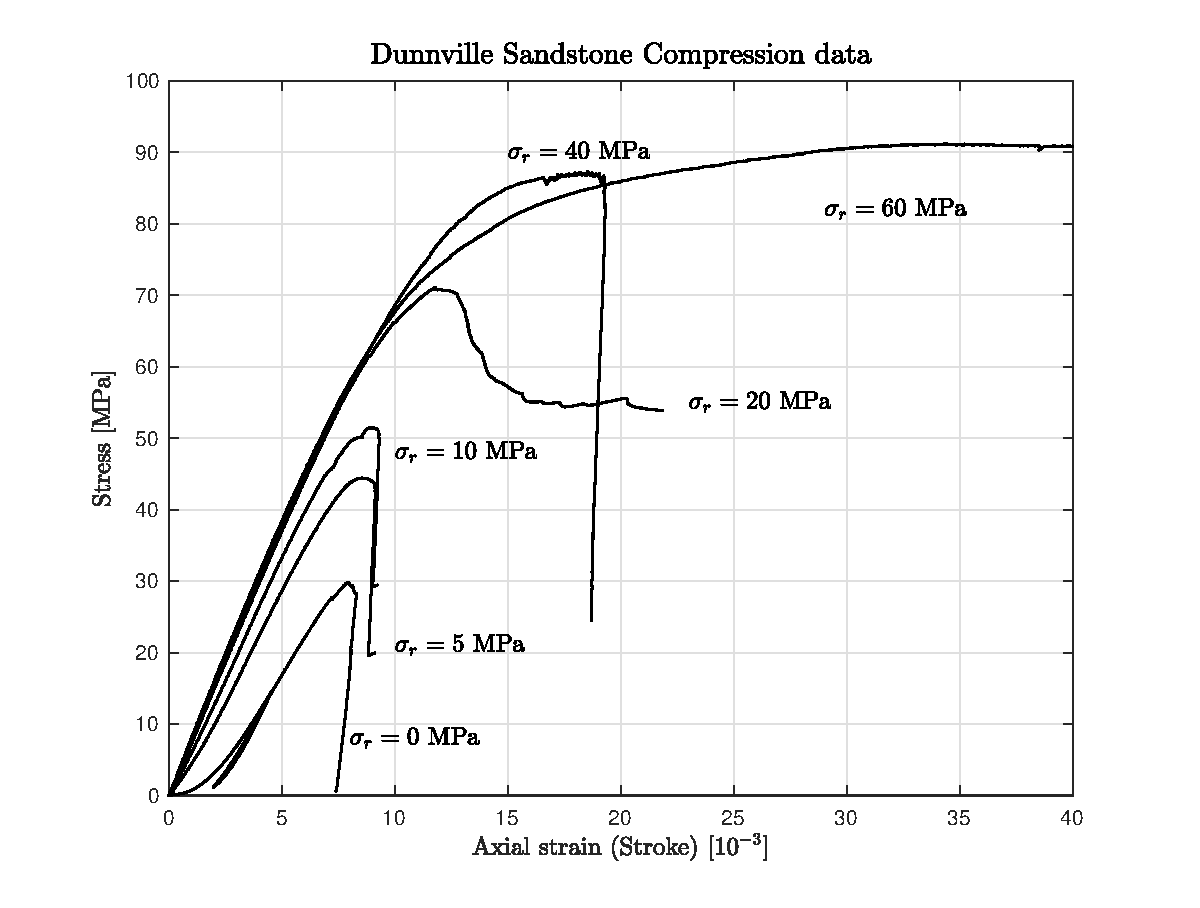
\includegraphics[width=\columnwidth]{ch3/CTC_summ}
    \caption{Summary of the stress-strain relationships for the triaxial compression and extension tests}
    \label{fig3:8}
\end{figure} 

\subsubsection{Conventional triaxial tests}

\paragraph{Stress vs. strain plot} From \SIrange{0}{20}{MPa} of confining stress, the rock is in the brittle domain as the axial stress is dropping after reaching its maximal strength. At higher confining pressures (i.e., $\sigma_r > 40 \si{MPa}$ and $\sigma_r < 60 \si{MPa}$), however, rock is transitioning from a brittle to ductile response as represented by the post-peak drop in stresses as seen in Fig. \ref{fig3:8}. Finally, the rock shows a ductile behavior under a confining stress of \SI{60}{MPa}, were the stress doesn’t reach a peak value, but keep increasing as multiple failure surfaces are created.

\paragraph{Mohr circles plot} 
The conventional triaxial compression results can also be presented using Mohr-Coulomb theory and particularly Mohr circles and their failure envelope. Fig. \ref{fig3:9} presents the Mohr circles of the five CTC tests. This plot indicates that the failure envelop for Dunnville sandstone is stress dependent and cannot be represented using the Mohr-Coulomb linear failure envelop for the entire range of possible stress states. The nonlinear failure envelop, however, may be linearized over small stress intervals as shown in Fig \ref{fig3:9}. The corresponding Mohr-Coulomb strength parameters (i.e., friction angle $\phi$  and cohesion intercept $c$) are summarized in Table \ref{tb3:MC-param}.

\begin{table}
    \centering
    \begin{tabular}{ccc}
        \hline
        Segment & [\si{\degree}] & $c$[\si{MPa}] \\
        \hline
        \hline
        5 – 10 MPa  & 30.73 & 9.67   \\ 
        10 – 20 MPa & 29.37 & 10.42  \\ 
        20 – 40 MPa & 14.41 & 23.6   \\ 
        40 – 60 MPa & 4.72  & 36.94  \\
        \hline
    \end{tabular}
    \caption{Mohr-Coulomb strength parameters for various stress regimes for Dunnville sandstone}
    \label{tb3:MC-param}
\end{table}

\begin{figure}[tb]
    \centering
    \includegraphics[width=\columnwidth]{ch3/mohrcoulomb}
    \caption{Mohr-Coulomb circles for the conventional triaxial compression tests.}
    \label{fig3:9}
\end{figure} 

\paragraph{Poisson’s ratio} 

The Poisson’s ratio of Dunnville Sandstone was computed using the results of the axial and radial strains for specimen TC 9:

\begin{equation}
    \nu = \frac{-\epsilon_{\text{radial}}}{\epsilon_{\text{axial}}} = 0.26
\end{equation}

Fig \ref{fig3:10} shows a plot of the radial strain vs. the axial strain measured during the test.

\begin{figure}[tb]
    \centering
    \includegraphics[width=\columnwidth]{ch3/poisson}
    \caption{poisson}
    \label{fig3:10}
\end{figure} 

\paragraph{Failure surfaces}

Table \ref{tb3:photoCTC} presents pictures of the CTC tests specimens after failure, where failure surfaces are observable. For all the tests, the failure angle is about \ang{60}, which correspond well to the theory associated with failure of isotropic rock under triaxial compression. 

\begin{table}
    \centering
    \begin{tabular}{|l|l|l|l|l|}
     \hline
     $\sigma_r = \SI{5}{MPa}$ & $\sigma_r = \SI{10}{MPa}$ &  $\sigma_r = \SI{20}{MPa}$ & $\sigma_r = \SI{40}{MPa}$ & $\sigma_r = \SI{60}{MPa}$ \\
     \hline
     \includegraphics[width=0.15\columnwidth]{ch3/ctc9-001.jpeg} & 
     \includegraphics[width=0.15\columnwidth]{ch3/CT_failAng-001} &
     \includegraphics[width=0.15\columnwidth]{ch3/CT_failAng-002} &
     \includegraphics[width=0.15\columnwidth]{ch3/CT_failAng-003} &
     \includegraphics[width=0.15\columnwidth]{ch3/ctc10} \\
     \hline
     $\theta = \ang{66}$ & $\theta = \ang{63}$  &  $\theta = \ang{57}$ & $\theta = \ang{58}$ & $\theta = $ ? \\
     \hline
    \end{tabular}
    \caption{Failure surfaces for conventional triaxial compression tests}
    \label{tb3:photoCTC}
\end{table}


\subsubsection{Conventional triaxial tests}

\paragraph{Stress vs. strain plot}

Fig \ref{fig3:8} also presents the stress vs. strain curves for the extension tests. The axial stress in the figure represent the amount of axial stress that is removed from the stress state. In order to find the axial stress at failure, the following formula is used: 

\begin{equation}
    \sigma_\text{failure} = \sigma_{a,\text{removed}} - \sigma_r
\end{equation}

The extension curves showed in the Fig. \ref{fig3:8} present a sudden increase in axial stress followed by a constant axial stress. This behavior is due to the failure of the specimen and particularly to the dilatancy of the specimen on the failure surface. As the failure surface is formed, the radial stress is higher than the axial stress and the confining pressure pushes the specimen out of the cell. The increase in axial stress is due to type of test performed, which is under displacement control. The load frame is still moving at the same rate, but the specimen is moved up against the load cell at a higher displacement rate. 

\paragraph{Failure surfaces}

Table \ref{tb3:photoCTE} presents pictures of the CTE tests specimens after failure. From Mohr-Coulomb theory, the expected orientation of the failure surface for isotropic rocks under triaxial compression is horizontal. The tested specimen show failures surfaces close to horizontal. The observable variations for \SI{35}{MPa} and \SI{60}{MPa} come from the small anisotropy due to the rock bedding, as the angles correspond to the bedding angles.  

\begin{table}
    \centering
    \begin{tabular}{|l|l|l|}
     \hline
     $\sigma_r = \SI{35}{MPa}$ & $\sigma_r = \SI{40}{MPa}$ &  $\sigma_r = \SI{60}{MPa}$ \\
     \hline
     \includegraphics[width=0.2\columnwidth]{ch3/CTE_failAng-003} & 
     \includegraphics[width=0.2\columnwidth]{ch3/CTE_failAng-001} &
     \includegraphics[width=0.2\columnwidth]{ch3/CTE_failAng-002} \\
     \hline
     $\theta = \ang{10}$ & $\theta = \ang{0}$  &  $\theta = \ang{27}$ \\
     \hline
    \end{tabular}
    \caption{Failure surfaces for conventional triaxial extension tests}
    \label{tb3:photoCTE}
\end{table}

